\makeatletter
\renewcommand{\chapter}{%
  \if@openright\cleardoublepage\else\clearpage\fi % Remove quebra padrão
  \secdef{\@chapter}{\@schapter}}
\makeatother
\chapter{Metodologia}
\label{metodo}

Este capítulo descreve as etapas metodológicas adotadas na condução do projeto de pesquisa. As atividades foram planejadas para garantir uma abordagem sistemática e consistente. A Figura \ref{fig-metodologia} ilustra o fluxo metodológico adotado.

\begin{figure}[h]
\centering
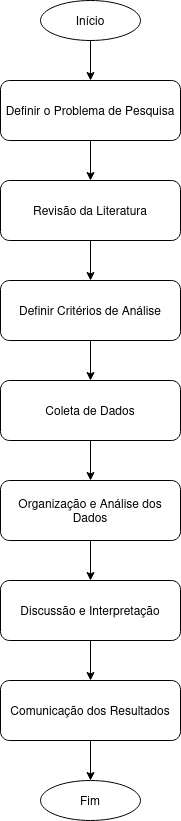
\includegraphics[width=0.3\textwidth]{imagem/metodologia.drawio.png}
\caption{Fluxo metodológico da pesquisa.}
\label{fig-metodologia}
\end{figure}


\section{Atividades a serem realizadas}
Nesta seção, detalhamos as atividades planejadas para o desenvolvimento do projeto.

\subsection{Atividade 1: Definir o problema de pesquisa}
A primeira atividade consiste na definição do problema de pesquisa, delimitando o tema e os objetivos específicos, com base em uma questão central que guiará o estudo.

\subsection{Atividade 2: Revisão da literatura}
A segunda atividade envolve uma revisão bibliográfica abrangente, buscando fundamentar teoricamente o problema e identificar lacunas na literatura.

\subsection{Atividade 3: Definir critérios de análise}
Nessa etapa, são estabelecidos os critérios que orientarão a coleta e análise dos dados, de forma a garantir consistência e validade no tratamento das informações.

\subsection{Atividade 4: Coleta de dados}
A coleta de dados será realizada utilizando técnicas específicas, como entrevistas, questionários ou análise documental, conforme o objetivo da pesquisa.

\subsection{Atividade 5: Organização e análise dos dados}
Os dados coletados serão organizados e analisados seguindo os critérios previamente definidos, utilizando métodos qualitativos e/ou quantitativos.

\subsection{Atividade 6: Discussão e interpretação}
Nessa etapa, os resultados obtidos serão discutidos e interpretados, relacionando-os aos objetivos iniciais e à literatura revisada.

\subsection{Atividade 7: Comunicação dos resultados}
Finalmente, os resultados serão comunicados por meio da elaboração de relatórios, artigos científicos e/ou apresentações.

\section{Cronograma}
A Tabela \ref{tab-crono} apresenta o cronograma das atividades descritas anteriormente, organizadas ao longo dos meses de execução do projeto.

\begin{table}[h]
\centering
\caption{Cronograma}
\label{tab-crono}
\begin{tabular}{|l|l|l|l|l|}
\hline
\textbf{Atividade} &
\textbf{\begin{tabular}[c]{@{}l@{}}Meses\\ 1-3\end{tabular}} &
\textbf{\begin{tabular}[c]{@{}l@{}}Meses\\ 4-6\end{tabular}} &
\textbf{\begin{tabular}[c]{@{}l@{}}Meses\\ 7-9\end{tabular}} &
\textbf{\begin{tabular}[c]{@{}l@{}}Meses\\ 10-11\end{tabular}} \\ \hline
Definição do problema & X &   &   &   \\ \hline
Revisão da literatura & X & X &   &   \\ \hline
Definir critérios      &   & X &   &   \\ \hline
Coleta de dados        &   &   & X &   \\ \hline
Análise dos dados      &   &   & X & X \\ \hline
Discussão              &   &   &   & X \\ \hline
Comunicação            &   &   &   & X \\ \hline
\end{tabular}
\end{table}
